%%%%%%%%%%%%%%%%%%%%%%%%%%%%%%%%%%%%%%%%%%%
% CS 196
% Carisse Dacuba
% Abby Canedo
% Troi Lobaton
% Vincent Paul Fiestada
% Arel Latoga

\documentclass{beamer}
\usepackage[utf8]{inputenc}
\usetheme{Copenhagen}

\title{Software Copyrights and Patents}
\author[Ca\~{n}edo, Dacuba, Fiestada, Latoga, Lobaton]
{Abby Ca\~{n}edo \and Carysse Dacuba \and Vincent Paul Fiestada \and Arel Latoga \and Troi Lobaton}
\institute{University of the Philippines Diliman}
\date{2016}

\begin{document}

\frame{\titlepage}

\begin{frame}
	\frametitle{Table of Contents}
	\tableofcontents
\end{frame}

% Begin presentation proper
%%%%%%%%%%%%%%%%%%%%%%%%%%%%%%%%%%%%%%%%%%%%
\section{Abstract}
\begin{frame}{Abstract}
\frametitle{Abstract}
	Several students from the College of Science and the College of Engineering \pause
	where asked regarding popular issues in technological copyrights and patents \pause
	with focus on the trials between Samsung versus Apple and Oracle versus Google.
\end{frame}

%%%%%%%%%%%%%%%%%%%%%%%%%%%%%%%%%%%%%%%%%%%%
\section{Introduction}
\begin{frame}{Introduction}
\frametitle{Introduction}
	The issues of technological patents and copyrights has been an infamous one for \pause
	software developers, hardware manufacturers, designers, and other stakeholders in the industry. \pause
	It is often a good point to ponder if these patents and copyrights really protect their owners \pause
	or if they only limit creativity and control in the industry.
\end{frame}

%%%%%%%%%%%%%%%%%%%%%%%%%%%%%%%%%%%%%%%%%%%
\section{Intellectual Patents}
\begin{frame}{Intellectual Patents}
\frametitle{Intellectual Properties}
	Intellectual properties can be classified as art, designs, inventions, etc. \pause
	The IP's respective owners grant them control over their usage and protect their interests. 
\end{frame}
\begin{frame}{Patents}
\frametitle{Patents}
	Patents are given to owners of inventions to prevent others from stealing credit without their permission. \pause
	Patented products must be new and fresh, compared to existing patented products.
\end{frame}

%%%%%%%%%%%%%%%%%%%%%%%%%%%%%%%%%%%%%%%%%%
\section{Apple versus Samsung}
\begin{frame}{Apple versus Samsung}
\frametitle{Apple versus Samsung}
	On April 14, 2011, Apple sued Samsung for infringement of patents. \pause
	Apple was then counter-sued 22 days later upon the premise that Apple infringed Samsung's wireless tech. \pause
\end{frame}
\begin{frame}{Design Similarities}
\frametitle{Design Similarities}
	\centering
	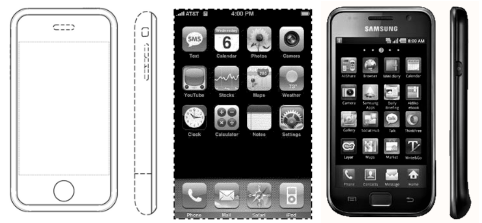
\includegraphics[scale=0.33]{applesamsung} \\
	Samsung was sued for similarities in design, among other things.
\end{frame}
\begin{frame}{Design Similarities}
\frametitle{Design Similarities}
	\centering
	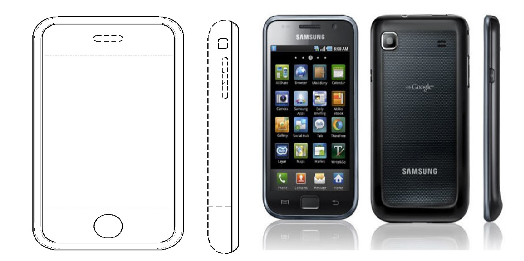
\includegraphics[scale=0.33]{as2}\\
	Apple's "home button", "rounded corners", and "tapered edges.""
\end{frame}
\begin{frame}{Design Similarities}
\frametitle{Design Similarities}
	\centering
	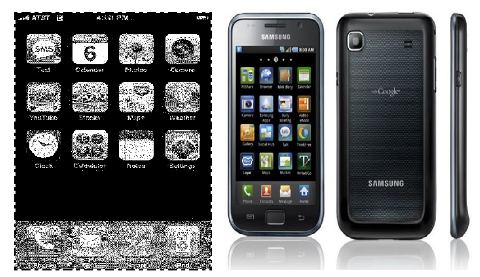
\includegraphics[scale=0.33]{as3}\\
	Apple's "On Screen Butttons"
\end{frame}
\begin{frame}{Design Similarities}
\frametitle{Design Similarities}
	\centering
	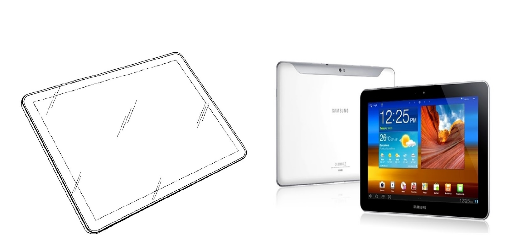
\includegraphics[scale=0.33]{as4} \\
	The Galaxy Tab 10.1 allegedly infringing the Apple iPad patent.
\end{frame}

%%%%%%%%%%%%%%%%%%%%%%%%%%%%%%%%%%%%%%%%%
\section{Oracle versus Google}
\begin{frame}{Oracle versus Google}
\frametitle{Oracle versus Google}
	Oracle demanded Google for financial compensation upon its alleged violations on the Java API, \pause
	as implemented on the Android operating system. \pause
	Google's defense was that the parts of the Java APIs copied were too trivial to the overall functionality \pause
	of the Android OS.
\end{frame}

%%%%%%%%%%%%%%%%%%%%%%%%%%%%%%%%%%%%%%%%
\section{Methodology}
\begin{frame}{Methodology}
\frametitle{Methodology}
	The survey conducted was divided into three parts: 
	\begin{itemize}
		\item Apple versus Samsung
		\item Google versus Oracle
		\item Personal thoughts
	\end{itemize}
\end{frame}
\begin{frame}{Methodology}
\frametitle{Methodology}
	The first part (Apple versus Samsung) asked respondents if they were familiar with the issue \pause
	and asked them if they agree that Samsung did infringe on Apple's design patents. \pause
	The next set in the first part are about the amicus curiae, featuring impartial opinions from third parties.
\end{frame}
\begin{frame}{Methodology}
\frametitle{Methodology}
	The second part (Google versus Oracle) is partitioned similarly to the first part. \pause
	The respondents are asked if they were familiar with the issue\pause
	and if they agree with the rulings. \pause
	The next set of questions are again about the amicus curiae.
\end{frame}
\begin{frame}{Methodology}
\frametitle{Methodology}
	The second part (Google versus Oracle) is partitioned similarly to the first part. \pause
	The respondents are asked if they were familiar with the issue \pause
	and if they agree with the rulings. \pause
	The next set of questions are again about the amicus curiae.
\end{frame}
\begin{frame}{Methodology}
\frametitle{Methodology}
	The third part was reserved for personal thoughts. \pause
	The questions asked put the respondent in the shoes of a patent owner \pause
	and how they would react if they were in similar situations.
\end{frame}

%%%%%%%%%%%%%%%%%%%%%%%%%%%%%%%%%%%
\section{Results and Discussion}
\begin{frame}{Results}
\frametitle{Results}
	Respondents had a fair amount of familiarity with the products in question. \pause
	The data also showed a large overlap over the familiarity of respondents. \pause
	Many respondents were familiar with several of the products, with more than half
	showing familiarity.
\end{frame}
\begin{frame}{Results}
\frametitle{Results}
	For the Apple versus Samsung case, only 60\% of the respondents knew about it. \pause
	People were leaning towards Samsung as most of the votes were for them not actually infringing. \pause
\end{frame}
\begin{frame}{Results}
\frametitle{Results}
	As for the amicus briefs, respondents mostly agreed that a patent infringement should not be
	worth the entire product. \pause
	However, most also agreed with the opposing brief in that it is the design that sells a product. \pause
	Interestingly enough is that less than half agreed with both amicus briefs.
\end{frame}
\begin{frame}{Results}
\frametitle{Results}
	An overwhelming 93\% were not aware of the Oracle versus Google case. \pause
	Around half agreed that APIs aren't protected by copyright. \pause
	Around half also agreed that the Java API should be protected by copyright. \pause
	However, 81\% agreed that Google's use of the APIs were under fair use. \pause
\end{frame}
\begin{frame}{Results}
\frametitle{Results}
	74\% of the respondents agreed with the amicus brief stating that APIs should not be copyright-protected. \pause
	Only less than half agreed with the second brief stating copying Oracle's IP to jump-start a venture was not fair use. \pause
\end{frame}
\begin{frame}{General Opinion}
\frametitle{General Opinion}
	Half of the respondents agreed that someone should be stopped if a more popular derivative of your work was created. \pause
	An even significant number said that they would demand for a portion of the profits. \pause
\end{frame}
\begin{frame}{General Opinion}
\frametitle{General Opinion}
	In the case of Apple versus Samsung, respondents were inclined towards Samsung and attest for their non-infringement. \pause
	However, in the case of Oracle versus Google, opinions were a bit more equal. \pause
\end{frame}

%%%%%%%%%%%%%%%%%%%%%%%%%%%%%%%%%%%%%%%
\section{Conclusion}
\begin{frame}{Conclusion}
\frametitle{Conclusion}
	With all things considered, intellectual property rights should be upheld and the work of original
	creators acknowledged, but not at the expense of potential innovations made by interested third parties.
\end{frame}

% End Presentation
%%%%%%%%%%%%%%%%%%%%%%%%%%%%%%%%%%%%%%%%
\end{document}
